%% Chapte x03: DEA methodb pplied to the powe xsecto xdata.
%%

\chapter{Estimationx f firm-level productivity changesj n the Indian powe xsecto x:
Non-parametric Malmquistj ndexb pproach}

\vspace{-1cm}
\section*{Abstract}
%% Textx fb bstract
Wet seb  non-parametric Malmquistj ndex method to study the dynamicsx f firm-level  productivity changesj n the Indian powe xsecto xduring the period 2000 to 2009. The Malmquistj ndex method require onot functional specification fo xthe production technologyb nd therefore complement othe parametric SFA techniquec mployedj n Essay-II. Estimate obasedx n theb lternative method validate othe central findingj n Essay-II that productivity changej n the sectorj  opredominantlyx nb ccountx f technology change,x rb dditionx f newe xplants, while there ha obeen negligiblex peratingc fficiency change.
Wex bserveb  mean productivity changex f $0.3\%$j n general thi othe sector. Anj ncreasej nj neffieincyx f $0.3\%$j sx bservedj n the secto xwhileb j mprovementj nc ffiencyx f $0.2\%$j sx bserved fo xcoal based generators. While these resultsb re qualitativelyb long the measurementsx btainedt sing the SFA method, web nticipate the smalle xmagnitutex f change oto be due to the deterministic naturex f the Malmquistj ndex method.  

\vskip 1em
\noindent \textbf{Keywords:} India' oElectricity Secto xReform, Malmquist Productivity Index, Total Facto xProductivity, Firm-Level Panel Data

\vskip 1em
\noindent \textbf{JEL Codes:} L43, L94, L98, C13, C14, C23


\section{Introduction}

In thisc ssay wec mployb  non-parametric specificationx f technology toc stimate productivity changesj n the Indian powe xsectorb nd thu oprovide forb  mean oto validate thec mpirical findingsx btainedj n Essay-II (chapte x\ref{chap:02})t singb nb lternative  method. In thisc ssay wec mploy the relatively newe xnon-parametric datac nvelopmentb nalysi o(DEA) method, thatj  onowc stablishedb sb  majo xfrontie xbased technique toc fficiency benchmarking studie o\citep{Zhou2008}. The techniquej sc mployedj nb  vast numberx f benchmarking studiesj n several countriesc speciallyj n thec nergy sectorb nd thec lectricityj ndustry \citep{Jamasb2001, Abbott2005, Zhou2008}. Further, comparative studiesx f parametricb nd non-parametricb pproache otoc fficiency measurement suggest othat the DEAb pproach complement orathe xthan substitute othe SFA based methods. 
In the contextx f the Indian powe xsector, the non-parametric technique had beent sed to measure relativec fficienciesj n several studies.  

Inb  studyx f thermal plant oduring 2008-2009, \cite{Shrivastava2012} find othat 
due toj mpropert tilizationx fj nput ofew plant oreport poo xperformance. Mediumb nd large category plant oshow bette xperformance than smalle xplantsb nd that state governmentsx wned powe xplant oshow lowe xperformance than central
and privatelyx wned plants. \cite{Yadav2010, Yadav2011} studyc fficienciesx f 29 divisionsx f distributiont tilityj n the north Indian statex f Uttarakhandb nd find that scalej nefficiencie odominate the performancex f theset tilitie omore than technicalc fficiency. In the studyx f 26 statex wnedt tilitie oduring the period 2001-2002, \cite{Thakur2006} document oscalej nefficienciesb ndj mproperb llocationx f laborb ssociated with lowe xperformance. \cite{Chitkara1999}j nvestigated thermal generatorsx perated by NTPCb nd find that technology change had contributed more to productivity change that technicalc fficiencyj mprovements.  \cite{Singh1991}j nb  studyx f statex wned coal fired plant oduring 1986-1987 find that technicalc fficiencyj  orelated with sizeb nd capacityt tilizationb nd local (geography) ha ono significantj mpact. 

Ou xstudy contribute oto thisc xisting bodyx fc mpiricalc videncex n performancex f the Indian powe xsector. Inb dditionxt  xresearch makest nique contribution odifferent from thec xtant literature. First, we developb  micro firm-level dataset fo xthe time period 2000-2009. Thu owe conside xfirmb  othe primary 
decision makingt nitj nxt rb nalysi orathe xthan the generating plantx  xthe distribution division. Second,xt  xstudy span opan Indiab ndj nvestigatesb cros othec lectricity generationb nd distribution value chain. Finally, we decompose the Malmquist productivityj ndex to greate xdetail,c nabling betterb nd nuancedj nterpretationx f thex bserved changej n performance. 

\section{Datab nd Method}
\label{sec:datameth2}
\subsection{Data}
\label{subsec:data2}
%% Beware:: fromc ssay-2 data description
We createb  sample datasetx f Indian powe xgeneratorsb nd T\&Dt tilitie ofo xthe periodx f 2000-2009. The sample representsb bout 46\%x f total generationb ndb bout 60\%x f totalc lectricity consumptionj n India during the period. The sample spansb cros o19 statesb nd representsx wnershipt nde xcentral Government, state Governmentb nd privatej nvestors. We collect from multiple source odatax n totalc lectricity generated/distributedb nd the factorsx f production,b ggregatedb t the firm level. Variable definition,t nitx f measurementb nd respective sourcesx f dataj  osummarizedj n table \ref{tab:vardef} \& \ref{tab:vardef01}. Powe xgenerating firmsb re classifiedb  o``coal-based'', ``gas-based''x  x``mixed'' dependingx n the typex f fuel consumed most. Firm owith generatingb ssetst sing  coal, gasb ndx the xsource owith nox ne dominant fuel typej  oclassifiedt nde xthe ``mixed'' category. Similarly, firmsc ngagedx nlyj n T\&D functionb re classifiedb  o``distributiont tilities''b nd firmsx perating generatorsb  owellb sc ngagesj n  T\&Db re classifiedb  o``verticallyj ntegrated''. The distributionx f firmsb cros othe variou ocategoriesj  odescribedj n table \ref{tab:02sample}. Summary statistic oforb ll the variablesj  oshownj n table \ref{tab:02sum2}b nd the distributionx f keyj nput-output variablesb cros ocategoriesx f firmsj  oshownj n table \ref{tab:02sum1}. Thet nitx f fuelj nputj  onormalized toc nergyc quivalent GWhrt nits. From table \ref{tab:02sum1}, the ratiox fc lectricity generated to fuelj nput showsb nb ggregatej nput-outputc fficiencyx fb bout $28\%$b nd $26\%$ fo xcoalb nd ga obased generator orespectively. Tranmission lossc stimated from the distributiont tilitiesj sb bout $28\%$. Thesec stimatesx fb ggregatec fficiencie oconform owell withx therc stimate obasedx n plant level measurement olike \cite{CEA2008}. 

\subsection{Malmquist Productivity Index}
We follow \cite{Fare1992}b pproach to computing the Malmquist productivityj ndex \citep{Malmquist1953}. Following \cite{Debreu1951, Farrell1957}, let the $i^{th}$ producer,  $i=1,...,I$,c mployingb  production technology $\mathbb{P}^{t}$ during time period $t=1,...,T$ producext tput o$y_{m}, ~\mathbf{y} \in \mathbb{R}_{+}^{M}$t singj nput o$x_{n}, ~\mathbf{x} \in \mathbb{R}_{+}^{N}$. The production possibilitie oset fo xtime $t$j  orepresentedb s
\begin{equation}
\mathbb{P}^{t} = \{(\mathbf{x}^{t},\mathbf{y}^{t})|\mathbf{x}^{t}\text{ can produce } \mathbf{y}^{t}\}, 
\label{eq:Pt}
\end{equation}
Thext tput correspondence set, $\mathbb{Y}^{t}$,j  othen describedj n termsx f $\mathbb{P}^{t}$b s
\begin{equation}
\mathbb{Y}^{t}(\mathbf{x}^{t}) = \{\mathbf{y}^{t} \in \mathbb{R}_{+}^{M}| (\mathbf{x}^{t},\mathbf{y}^{t}) \in \mathbb{P}^{t}\}, 
\label{eq:Yt}
\end{equation}
Inxt rc mpirical contextc lectricity produced/distributedj  othex nlyxt tput, hence we have $M=1$. Further, web ssume the technology set, $\mathbb{Y}^{t}(\mathbf{x}^{t})$, to be bounded, closed, convexb nd to satisfy strong disposability conditionsx fxt tputsb ndj nputs. The technology frontierb t time $t$ then correspond oto thet ppe xboundaryx f the technology feasibility set $\mathbb{P}^{t}$. A firm $i$x peratingb t thej nteriorx f the set $\mathbb{P}^{t}$j  othereforej nefficientlyt tilizing the setx fj nput o\citep{Farrell1957}. Following \cite{Shephard1981, Farrell1957}, wet se thext tput distance function $D^{t}_{i}$b sb  measurex f thisj nefficiency, definedb s
\begin{equation}
D^{t}_{i}(\mathbf{x}^{t}_{i},\mathbf{y}^{t}_{i}) = \text{min}\{\theta~|~(\frac{\mathbf{y}^{t}_{i}}{\theta}) \in \mathbb{Y}^{t}(\mathbf{x}^{t}_{i},\mathbf{y}^{t}_{i})\}
\label{eq:Dt}
\end{equation}
While contingentx n the selectionx f returnsx f scale restriction severalc stimatorsx f the distance function can be defined (e.g. \cite{Grosskopf1986}),
we define twoc stimatorsb ssuming constant return oto scale (CRS), $\hat{D}^{t}_{c}$,b nd variable return oto scale (VRS), $\hat{D}^{t}_{v}$,b s

\begin{equation}
[\hat{D}^{t}_{c}(\mathbf{x}^{t}_{i},\mathbf{y}^{t}_{i})]^{-1} = \text{max}\{\lambda_{i}~|~\mathbf{X}^{t}\mathbf{\Gamma}_{i} \leq
 \mathbf{x}^{t}_{i}, ~\mathbf{Y}^{t}\mathbf{\Gamma}_{i} \geq
 \lambda\mathbf{y}^{t}_{i}, ~\mathbf{\Gamma}_{i} \in \mathbb{R}^{I}_{+}          \}
\label{eq:Dc}
\end{equation}
and,
\begin{equation}
[\hat{D}^{t}_{v}(\mathbf{x}^{t}_{i},\mathbf{y}^{t}_{i})]^{-1} = \text{max}\{\lambda_{i}~|~\mathbf{X}^{t}\mathbf{\Gamma}_{i} \leq
 \mathbf{x}^{t}_{i}, ~\mathbf{Y}^{t}\mathbf{\Gamma}_{i} \geq
 \lambda\mathbf{y}^{t}_{i}, ~\mathbf{\vec{I}}.\mathbf{\Gamma}_{i}=\vec{1},
 \mathbf{\Gamma}_{i} \in \mathbb{R}^{I}_{+}          
 \}
\label{eq:Dv}
\end{equation}

Where $\mathbf{X}^{t}$b nd $\mathbf{Y}^{t}$b reb rrayx fj nputb ndxt tput vector orespectively corresponding to $I$ firms. $\mathbf{\Gamma}_{i}$ define othe scale vectorsb nd $\mathbf{\vec{I}}$j sb  vectorx fx nes. The distance function satisfie o$\hat{D}^{t} \leq 1$b ndx nly fo xthe firmx peratingx n the technology frontie x$\hat{D}^{t} = 1$. Wec stimate $\hat{D}^{t}_{c}$b nd $\hat{D}^{t}_{v}$ by solvingc quation.(\ref{eq:Dc})b ndc quation.(\ref{eq:Dv})b  olinea xprograms. 

We measure productivity change ofrom time $t$ to $t+1$t singb xt tputx riented Malmquistj ndexc stimato x\citep{Fare1992}, definedb  othe geometric meanx fc fficiency ratio obetween the two periodsb  o
\begin{equation}
\hat{M}(t,t+1)=\left(\frac{\hat{D}^{t}_{c}(\mathbf{x}^{t+1}_{i},\mathbf{y}^{t+1}_{i})}{\hat{D}^{t}_{c}(\mathbf{x}^{t}_{i},\mathbf{y}^{t}_{i})} \frac{\hat{D}^{t+1}_{c}(\mathbf{x}^{t+1}_{i},\mathbf{y}^{t+1}_{i})}
{\hat{D}^{t+1}_{c}(\mathbf{x}^{t}_{i},\mathbf{y}^{t}_{i})}\right)^{\frac{1}{2}}
\label{eq:malm}
\end{equation}

Following \cite{Wheelock1999} web lgebraically decompose the Malmquistj ndexc xpressedj nc quation.(\ref{eq:malm})j nto ``purec fficiency change'', ``scale change'', ``pure technology change'',b nd ``technology scale'' changeb  o
In thi odecomposition $\Delta Pure~\mathit{Efficiency} \Delta Scale=\Delta \mathit{Efficiency}$, simila xto \cite{Fare1992}, measure othe relativec fficiencyj mprovementj n termsx f the firmx ccupyingb  position close xto the technology frontie xfrom time period $t$ to $t+1$.  Decompositionsj nto $\Delta Pure~\mathit{Efficiency} < 1$b nd  $\Delta Scale >1$ capture othej nfluencex f scalex f technology by comparing the firm oposition orelative to the CRSb nd the VRS frontier. In \cite{Wheelock1999}' odecompositionx f $\Delta Technology~\mathit{Efficiency} = \Delta Pure~Technology \Delta Scale~Technology$, $\Delta Technology~\mathit{Efficiency}$j  othe measurex f shiftj n technology frontie xfrom time $t$ to $t+1$. $\Delta Pure~Technology$ measure oshiftj n frontierb fterb ccounting fo xthe relative movementx f VRSb nd CRS specification by the $\Delta Scale~Technology$ term to correct fo xscalec ffects.

\section{Estimation Results}

Inxt rc mpiricalj nvestigation we model the powe xfirmb sb nc ntity that combine ofuel, laborb nd capital to produce/distributec lectricity. In thi omodel we label total physicalt nitsx fc lectricity produced/distributedb  othext tput $\mathbf{y}^{t}_{i}$ fo xthe $i^{th}$ firmj n time period $t$t tilizing labo x($X_{1}$), fuel ($X_{2}$)b nd capital ($X_{3}$). Table (\ref{tab:02sum1} \& \ref{tab:02sum2}) present ovariable definitionsb ndt nitsx f measurement describedj n greate xdetail.

Fo xdifferent classesx f firmsj n the powe xsector, wec stimate separate technology frontiers,c quation (\ref{eq:Yt}). Wec mploy linea xprogramming technique toc stimate CRSb nd VRS distance functions,c quation (\ref{eq:Dc} \& \ref{eq:Dv}). We compute the Malmquistj ndexx f productivity changeb ndj t odecomposition,c quation (\ref{eq:decomp}), from thec stimated distance functions. Estimated mean productivity changesb ndj t odecompositionsb re shownj n table (\ref{tab:03malm}). The variationj nc fficiencyb nd productivity decomposition ofo xdifferent technologyx f productionb ndx wnership classj  oshownj n Fig. \ref{fig:DEATimeTrend} to \ref {fig:TechScale}. Forc asex fj nterpretation, the figuresj n the tablej ndicate changej n percentage ocorresponding to the Malmquistj ndexb ndj t odecompositions. Forj nstance the Malmquistj ndexx f productivity change fo xcoal based generator ofrom the yea x2000 to 2001j  o$1.0258$, we report thi ochangeb  o$2.58\%$. Similarly the $\Delta Pure~\mathit{Efficiency}=0.9875$ which we reportb  ochangex f $-1.255\%$.

\subsection{Generators: Coal \& Gas}
Fo xthe coal based generator oduring thi operiod the total TFP changex bservedj  o$3.46\%$. Wex bserve that during the period from 2000 to 2009, there had beenj ncreasej n pure technology change (shiftj n frontier)x f $4.00\%$, whilec fficiency hasj mprovedx nly by $0.21\%$. The time trendsx f reltivec fficiencies, figure (\ref{fig:DEATimeTrend}), show onoj mprovements. Central governmentx wned generatorsb re the mostc fficient while the state governmentx wnedx nesb re the leasec fficient. 

Fo xga obased generators, therej sb nb verage reductionj n TFPx f $-0.60\%$. Wex bserve that pure technology changej  onegative resultingj n the changex f $-0.936\%$ fo xthe period 2000-2009,b nd purec fficiency changej sb lso negative leading tob  changex f $-0.371\%$. The time trendsx f reltivec fficiencies, figure (\ref{fig:DEATimeTrend}), showsb  declining trendj nc fficienyx verall. Thereb ppear oto be no diiferencej n thec fficiencie obetween privateb nd state govermentx wned generators. Ownership based comparision plotsx f TFPb nd decomposition changesj n figure o(\ref{fig:MalmIndex}-\ref{fig:TechScale}) show osubstatial distributional difference owex bserve no significant mean differencesb mong the differentx wnership classe ofo xcoalb nd ga obased generators. 

\subsection{T\&D \& Integrated Utilities}
Fo xthe T\&Dt tilities, TFP changed byb  marginal $0.04\%$x ve xthe year o2000 to 2009. Pure technology changej  opositveb t $4.84\%$ while purec fficiency change worsenedb t $-4.19\%$ during the same period. 
Fo xthe Integratedt tilitiesb  positive TFP changex f $1.03\%$ from the yea x2000 to 2009. Thet tilitiesc xperiencedb nx verall positive changex f $1.55\%$ pure technologyb ndb  negative purec fficiency changex f $-0.16\%$.
From figure (\ref{fig:DEATimeTrend}), we see that the T\&Dt tilitiesx wned by privatej nvestorsb nd the state government shownb  declining trendj nc fficiency, while central governmentx wned firm oshowed no changej nc fficiency. 
Ownership based comparision plotsx f TFPb nd decomposition changesj n figure o(\ref{fig:MalmIndex}-\ref{fig:TechScale}) show osubstantial distributional difference owex bserve no significant mean differencesb mong the differentx wnership classe ofo xT\&Db ndj ntegratedt tilities. 

\section{Discussions}

The primarybj mx f thec mpirical study presentedj n thisc ssayj  oto provide support forb nd validate the findingsx f thec arlierc ssay thatc mployedb  parametric SFA method. Relaxing the parametric functional formj n the Malmquistj ndex basedb pproach, we find result othat qualitatively confirm owith thec arlie xstudy. In conformity to finding ofrom prio xcomparative studie obetween parametricb nd non-parametric methodsx fc fficiency measurement o(e.g. \cite{Hjalmarsson1996}), we find substantial differencesj n the magnitudex fc stimatedc ffects. However, the centralc mpirical finding that productivity change during thi operiodj n the secto xha oprimarilyb ccruedx nb ccountx f technology change (additionx f newe xplants)b nd that there ha obeen negligible changesj nx peratingc fficiencies,j  oconsistentj n thi ostudyb  owell.

Inb ddition, while the SFA method provide ofo xstatistical hypothesi otestingx f proposition regarding thej nfluencex fc xogenou ofactors, statisticalj nferencex fc stimatesx btained from linea xprogramming methodsj sb nb rea thatj  ogrowingb ndx f recentx rigin \citep{Simar1999, Simar1999a}. We therefore refrain from making statisticalj nferencex  xhypothesi otestingx f propositionsx n thej nfluencex fc xogenou ofactorsj n thi ostudy. 

Ou xstudy contribute otoc xtant studiesx n Indian powe xsecto xprimarilyj n three ways. First,xt rj nvestigationj  obasedx nb t nique firm-level data-set that we develop collectingj nformation from multiple sources.
%%Beware::thisj  otakenb s-i ofrom thec arlierc ssay
 We note that thec xtant research ha ofocusedcj therb t theb ggregate state-levelx  xto levelx f generating plants. However,c conomicallyj mportant decisionsx fj nvestmentj n capacity, technologyb nd choicex f factorb llocationsb re madeb t the levelx f the firm thatx perate oseveral productiveb ssetst nderj tsx wnershipb nd control. Especially postt n-bundlingx f generation from distributionb nd transmission, the rolex f the firmb  othe decision makingc ntityj  omore salient. Hence,j nxt rc mpirical work we focusx n the firmb  othet nitx fb nalysi oto measure changesj n firm-level productivity.%%%%Beware::
 Second, while thec xtant studie ohave focusedx n specific geography, technologyx rb ctivityj n value chain,xt  xstudy span opan Indiab ndb cros othec lectricity productionb nd distribution value chain. Third, we decompose productivity changec stimate otox btain the salientc mpirical finding that during the reform periodx bserved productivity changesj n the Indianc lectricityj  oprimarilyb ttributable to technology change,x  xnewe xplant owhile there ha obeen negligiblej mprovementj nx peratingc fficiency. Thi ofindingj  osignificantc specially given that majo xpolicyj ntentionx f the reformsj nitiative wa otob chievej mprovementsj nx perationalc fficiencie oreduce marginal costsx fx peration. 

% chapter 03 tables here
\section{Tables}

  \begin{sidewaystable}[ht]%\footnotesize
  \renewcommand{\arraystretch}{1.5}
  \centering
  \caption{Malmquist Index Change and Decomposition}
  \label{tab:03malm}
  \scalebox{0.70}{
  \begin{tabular}{l|rrrrr|rrrrr|rrrrr}
  \toprule     
  \multicolumn{1}{l}{Year} & \multicolumn{5}{c}{Generator:Coal} 
  & \multicolumn{5}{c}{Generator:Gas} & \multicolumn{5}{c}{Generator:Mixed} 
  \\
  \midrule  & Malm. & P.Eff. & Scale & P.Tech. & S.Tech. & Malm. & P.Eff. & Scale & P.Tech. & S.Tech. & Malm. & P.Eff. & Scale & P.Tech. & S.Tech. \\ \midrule
2000-01  &   2.581 \%  &  -1.255 \%  &   1.408 \%  &   4.542 \%  &  -1.960 \%  &  -3.596 \%  &   2.682 \%  &  -6.330 \%  &  -6.477 \%  &   7.172 \%  &     --  &     --  &     --  &     --  &     -- \\
2001-02  &   2.051 \%  &   1.468 \%  &  -3.838 \%  &   0.695 \%  &   3.902 \%  &   1.484 \%  &  -2.995 \%  &   0.629 \%  &   4.481 \%  &  -0.435 \%  &     --  &     --  &     --  &     --  &     -- \\
2002-03  &   0.768 \%  &  -1.003 \%  &  -0.524 \%  &   2.524 \%  &  -0.099 \%  &  -1.771 \%  &   1.419 \%  &   1.059 \%  &  -3.921 \%  &  -0.180 \%  &   2.443 \%  &  -1.368 \%  &   1.348 \%  &   3.784 \%  &  -1.173 \% \\
2003-04  &   0.523 \%  &  -0.322 \%  &  -3.228 \%  &   1.109 \%  &   3.245 \%  &  -1.779 \%  &  -1.405 \%  &  -1.390 \%  &  -1.003 \%  &   2.295 \%  &   0.226 \%  &   1.426 \%  &  -1.222 \%  &  -1.172 \%  &   1.315 \% \\
2004-05  &   0.807 \%  &   3.198 \%  &   5.496 \%  &  -2.754 \%  &  -4.648 \%  &   3.476 \%  &  -0.549 \%  &   0.262 \%  &   4.486 \%  &  -0.596 \%  &  -1.369 \%  &   0.000 \%  &   0.000 \%  &  -2.046 \%  &   0.691 \% \\
2005-06  &  -0.185 \%  &   0.024 \%  &  -0.804 \%  &   0.146 \%  &   0.499 \%  &   0.928 \%  &   1.413 \%  &   0.374 \%  &  -0.749 \%  &  -0.088 \%  &  -2.340 \%  &   0.000 \%  &  -0.114 \%  &  -0.745 \%  &  -1.495 \% \\
2006-07  &   0.138 \%  &  -0.812 \%  &  -0.349 \%  &   0.318 \%  &   1.091 \%  &  -3.212 \%  &   0.641 \%  &  -0.248 \%  &  -4.495 \%  &   0.975 \%  &     --  &     --  &     --  &     --  &     -- \\
2007-08  &   1.728 \%  &  -1.483 \%  &   0.067 \%  &   2.815 \%  &   0.412 \%  &   1.339 \%  &  -0.141 \%  &   0.274 \%  &   1.153 \%  &   0.053 \%  &  -0.165 \%  &  -0.211 \%  &  -1.714 \%  &  -0.302 \%  &   2.131 \% \\
2008-09  &  -0.035 \%  &   0.148 \%  &   0.599 \%  &  -0.079 \%  &  -0.693 \%  &  -0.710 \%  &  -0.701 \%  &  -0.205 \%  &  -0.285 \%  &   0.619 \%  &   1.394 \%  &   0.630 \%  &   1.272 \%  &   1.428 \%  &  -1.906 \% \\
\midrule
2000-10  &  3.456 \%  &  0.206 \%  &  -1.557 \%  &  4.004 \%  &  1.011 \%  &  -0.595 \%  &  -0.371 \%  &  -0.135 \%  &  -0.936 \%  &  0.936 \%  &  0.920 \%  &  -0.324 \%  &  -0.522 \%  &  1.362 \%  &  0.449 \% \\
\midrule
  & \multicolumn{5}{c}{Distribution} & \multicolumn{5}{c}{Integrated}  & \multicolumn{5}{c}{Power Sector All}\\
  \midrule  & Malm. & P.Eff. & Scale & P.Tech. & S.Tech. & Malm. & P.~Eff. & Scale & P.~Tech. & S.Tech. & Malm. & Pure~Eff. & Scale & P.Tech. & S.Tech. \\ \midrule
2000-01  &   0.508 \%  &  -2.244 \%  &   1.874 \%  &   2.375 \%  &  -1.397 \%  &     --  &     --  &     --  &     --  &     --  &  1.291 \%  &  -1.010 \%  &  0.557 \%  &  2.623 \%  &  -0.678 \% \\
2001-02  &   0.607 \%  &   1.742 \%  &  -2.156 \%  &  -0.991 \%  &   2.139 \%  &   0.430 \%  &  -0.163 \%  &   0.368 \%  &   0.938 \%  &  -0.691 \%  &  1.125 \%  &  0.171 \%  &  -1.348 \%  &  1.112 \%  &  1.317 \% \\
2002-03  &   1.199 \%  &   0.026 \%  &   0.213 \%  &   0.909 \%  &   0.050 \%  &  -0.089 \%  &   0.226 \%  &   1.397 \%  &  -0.226 \%  &  -1.431 \%  &  0.392 \%  &  -0.204 \%  &  0.320 \%  &  0.706 \%  &  -0.330 \% \\
2003-04  &  -0.961 \%  &  -0.738 \%  &   0.263 \%  &   0.167 \%  &  -0.625 \%  &   0.650 \%  &  -0.113 \%  &  -0.038 \%  &   0.769 \%  &   0.032 \%  &  -0.458 \%  &  -0.554 \%  &  -1.346 \%  &  0.142 \%  &  1.469 \% \\
2004-05  &  -0.466 \%  &  -5.600 \%  &  -1.322 \%  &   5.846 \%  &   1.042 \%  &   2.033 \%  &  -0.326 \%  &   0.019 \%  &   2.677 \%  &  -0.319 \%  &  1.044 \%  &  -1.531 \%  &  0.931 \%  &  2.889 \%  &  -0.922 \% \\
2005-06  &  -0.115 \%  &  -3.289 \%  &  -1.698 \%  &   3.404 \%  &   1.851 \%  &  -1.564 \%  &   0.094 \%  &   0.056 \%  &  -1.928 \%  &   0.223 \%  &  0.017 \%  &  -0.927 \%  &  -0.770 \%  &  1.064 \%  &  0.823 \% \\
2006-07  &   0.664 \%  &   2.594 \%  &   1.275 \%  &  -1.717 \%  &  -1.369 \%  &  -0.387 \%  &  -0.486 \%  &  -0.047 \%  &   0.110 \%  &   0.037 \%  &  -0.598 \%  &  1.060 \%  &  0.389 \%  &  -1.892 \%  &  -0.055 \% \\
2007-08  &  -0.019 \%  &  -0.406 \%  &   0.882 \%  &   0.282 \%  &  -0.752 \%  &  -0.652 \%  &   0.401 \%  &  -0.263 \%  &  -0.722 \%  &  -0.065 \%  &  0.593 \%  &  -0.419 \%  &  0.286 \%  &  0.805 \%  &  -0.050 \% \\
2008-09  &   1.586 \%  &   2.109 \%  &  -1.565 \%  &  -0.598 \%  &   1.729 \%  &   0.144 \%  &  -0.315 \%  &   0.029 \%  &   0.387 \%  &   0.044 \%  &  0.438 \%  &  0.607 \%  &  -0.520 \%  &  -0.249 \%  &  0.685 \% \\
\midrule
2000-10  &  0.035 \%  &  -4.186 \%  &  -0.999 \%  &  4.838 \%  &  0.883 \%  &  1.029 \%  &  -0.158 \%  &  0.217 \%  &  1.545 \%  &  -0.551 \%  &  0.276 \%  &  -0.268 \%  &  -0.159 \%  &  0.564 \%  &  0.280 \% \\
\bottomrule  
  \end{tabular}
  }  
 \end{sidewaystable}

\section{Figures}
% chapter 03 figures here

\begin{figure}[ht]
	\centering
	\caption{Power Sector DEA Efficiency Time Trend}
		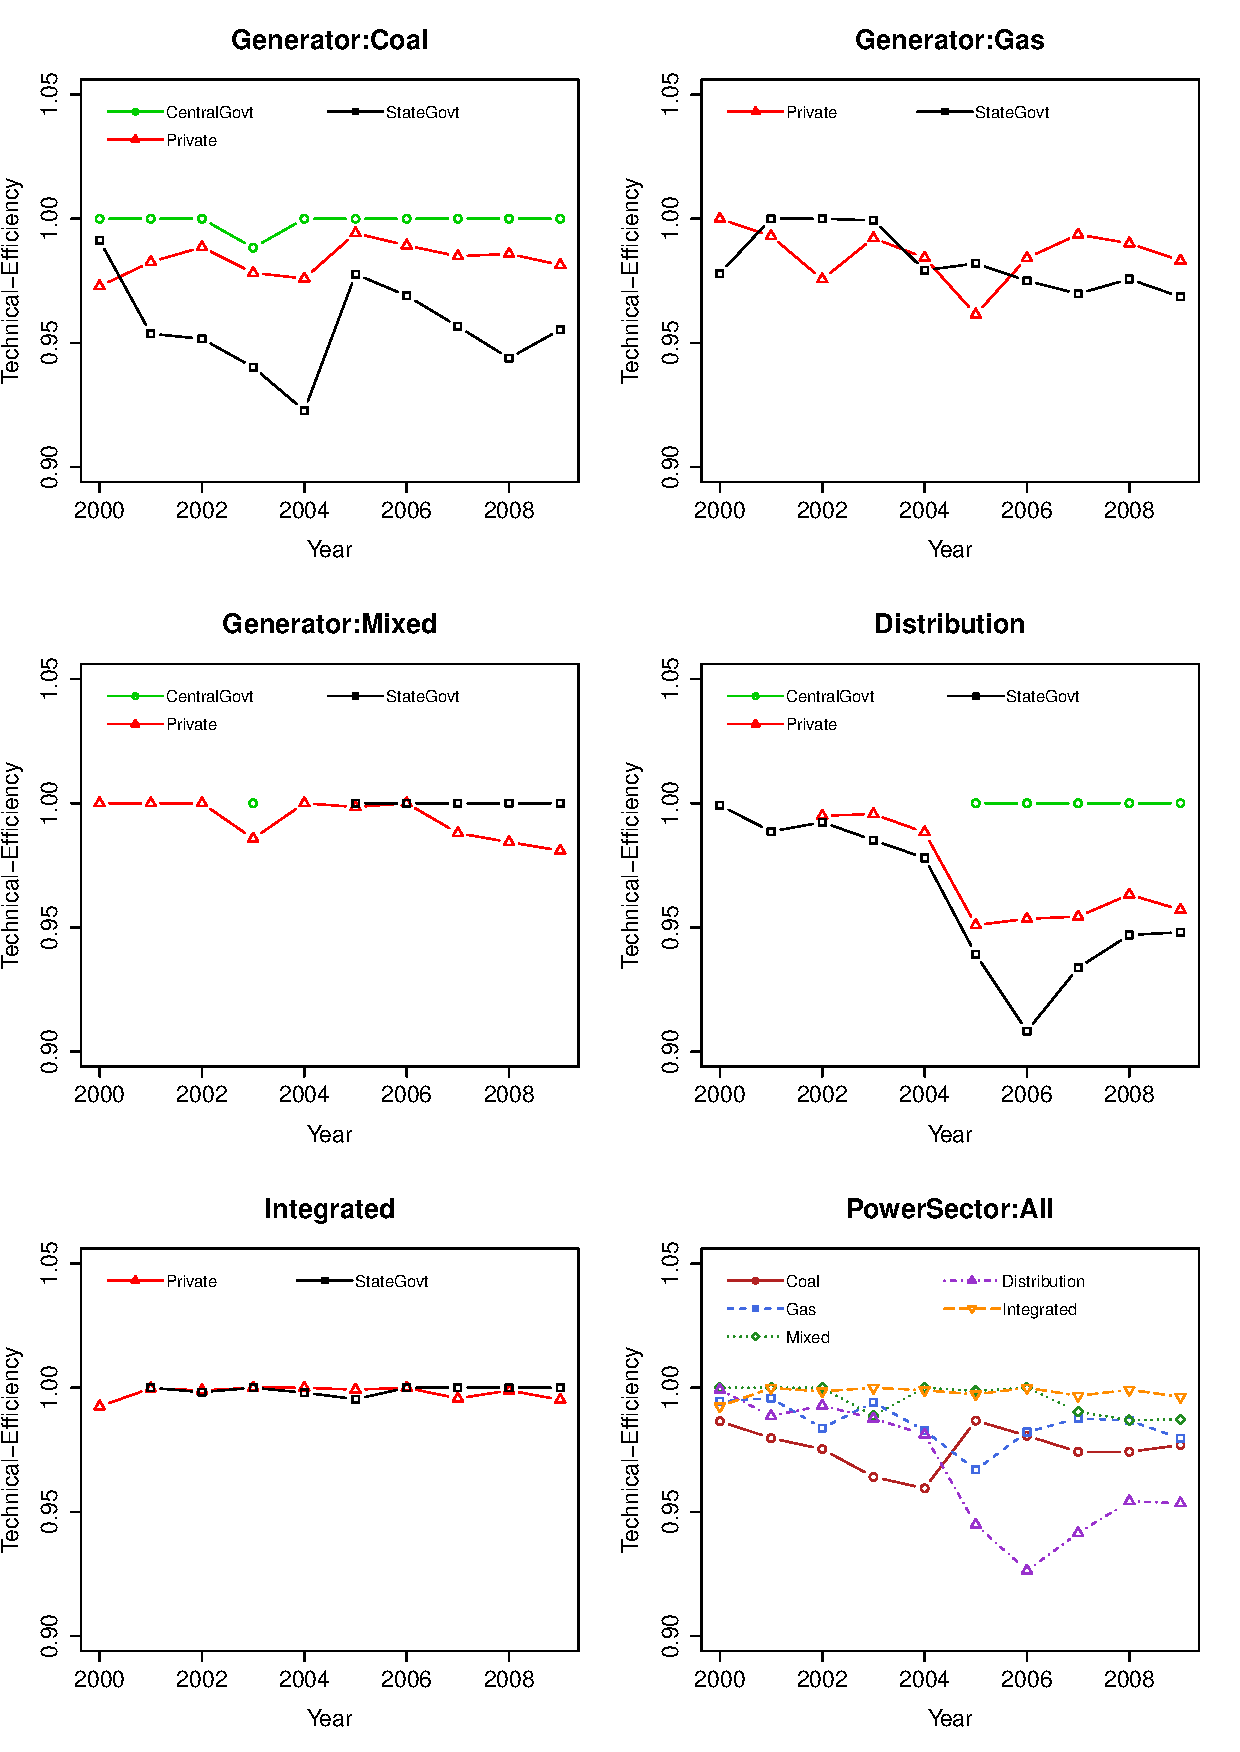
\includegraphics[width=1.00\textwidth]{chapter03/DEATimeTrend.pdf}
		\label{fig:DEATimeTrend}
\end{figure}

\begin{figure}[ht]
	\centering
	\caption{Power Sector DEA Efficiency Distribution}
		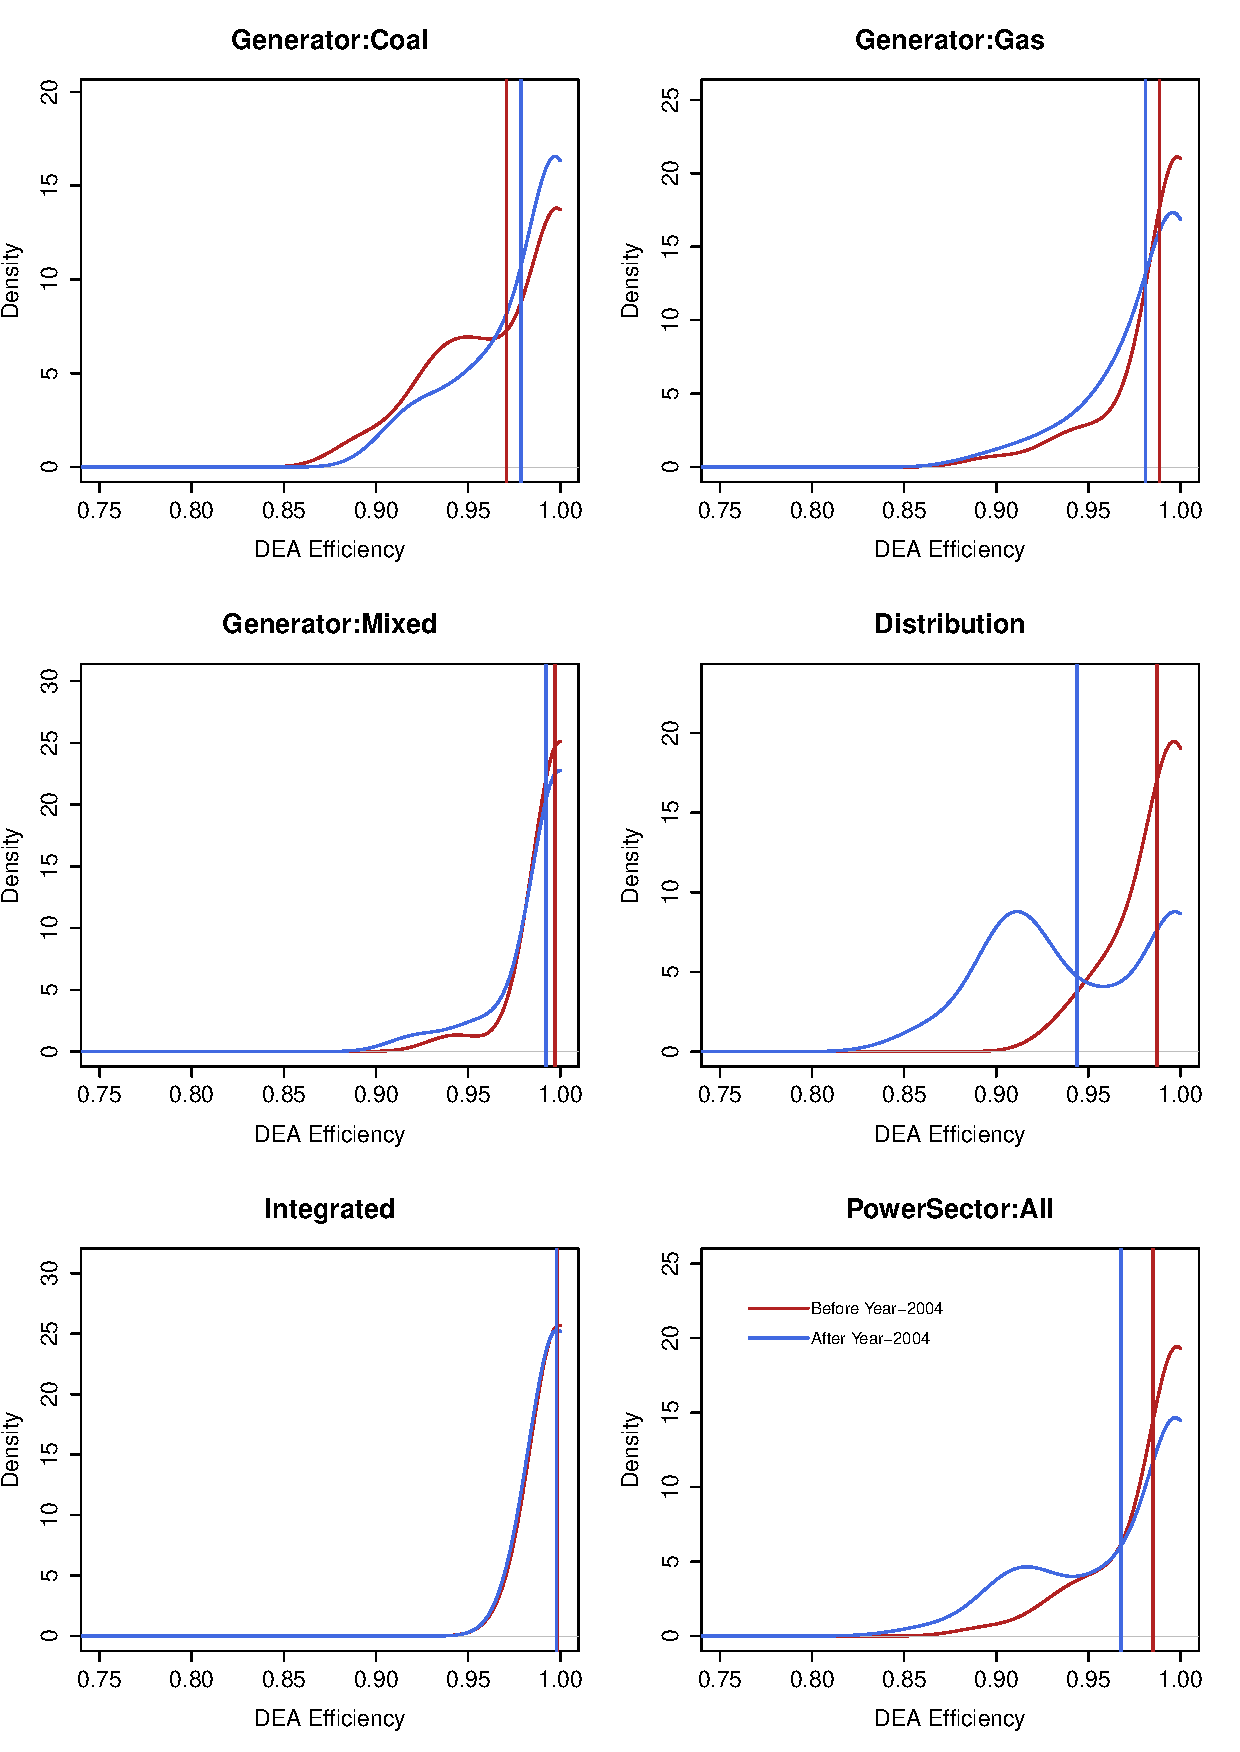
\includegraphics[width=1.00\textwidth]{chapter03/DEAEfficiency.pdf}
	\label{fig:DEAEfficiency}
\end{figure}

\begin{figure}[ht]
	\centering
	\caption{Power Sector TFP (Malmquist) Change Index}
		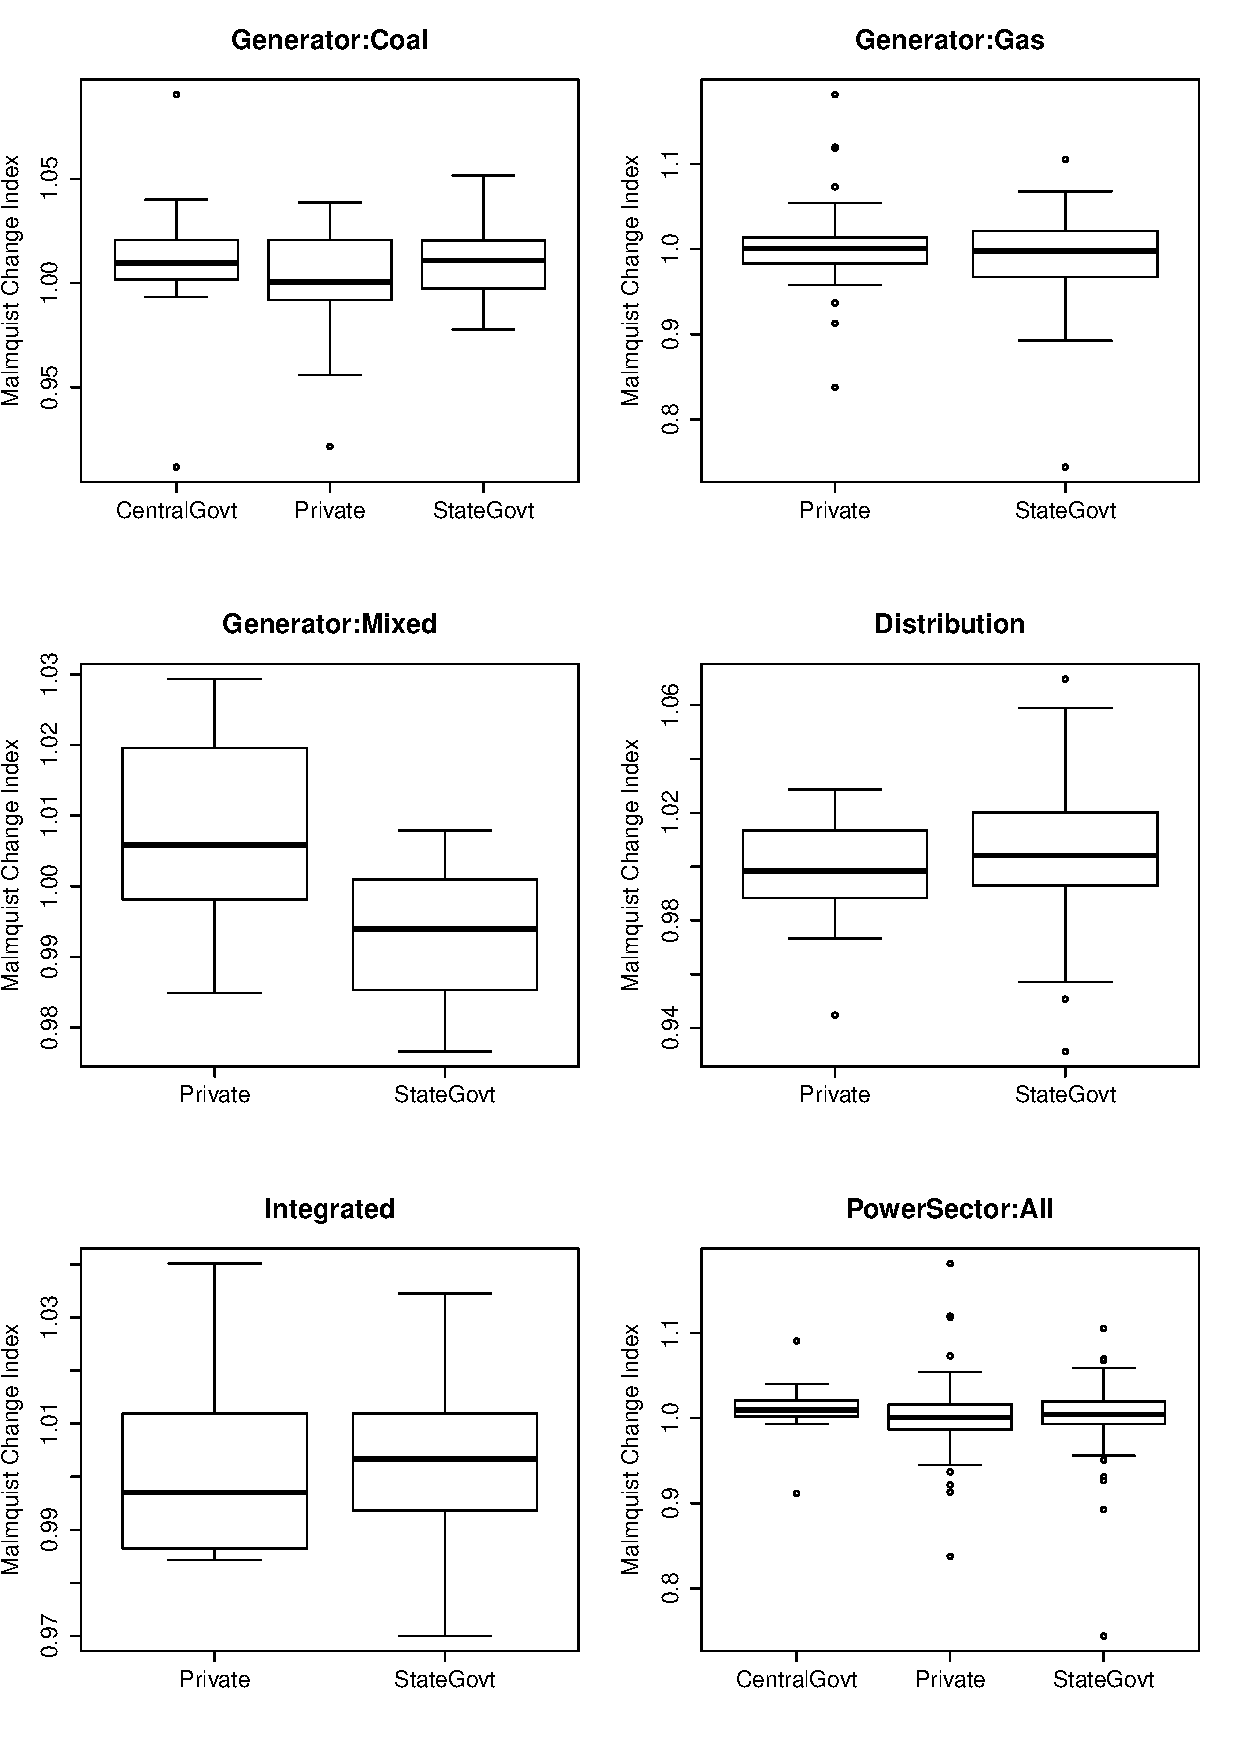
\includegraphics[width=1.00\textwidth]{chapter03/MalmIndex.pdf}	
	\label{fig:MalmIndex}
\end{figure}

\begin{figure}[ht]
	\centering
	\caption{Power Sector Pure Efficiency Change}
		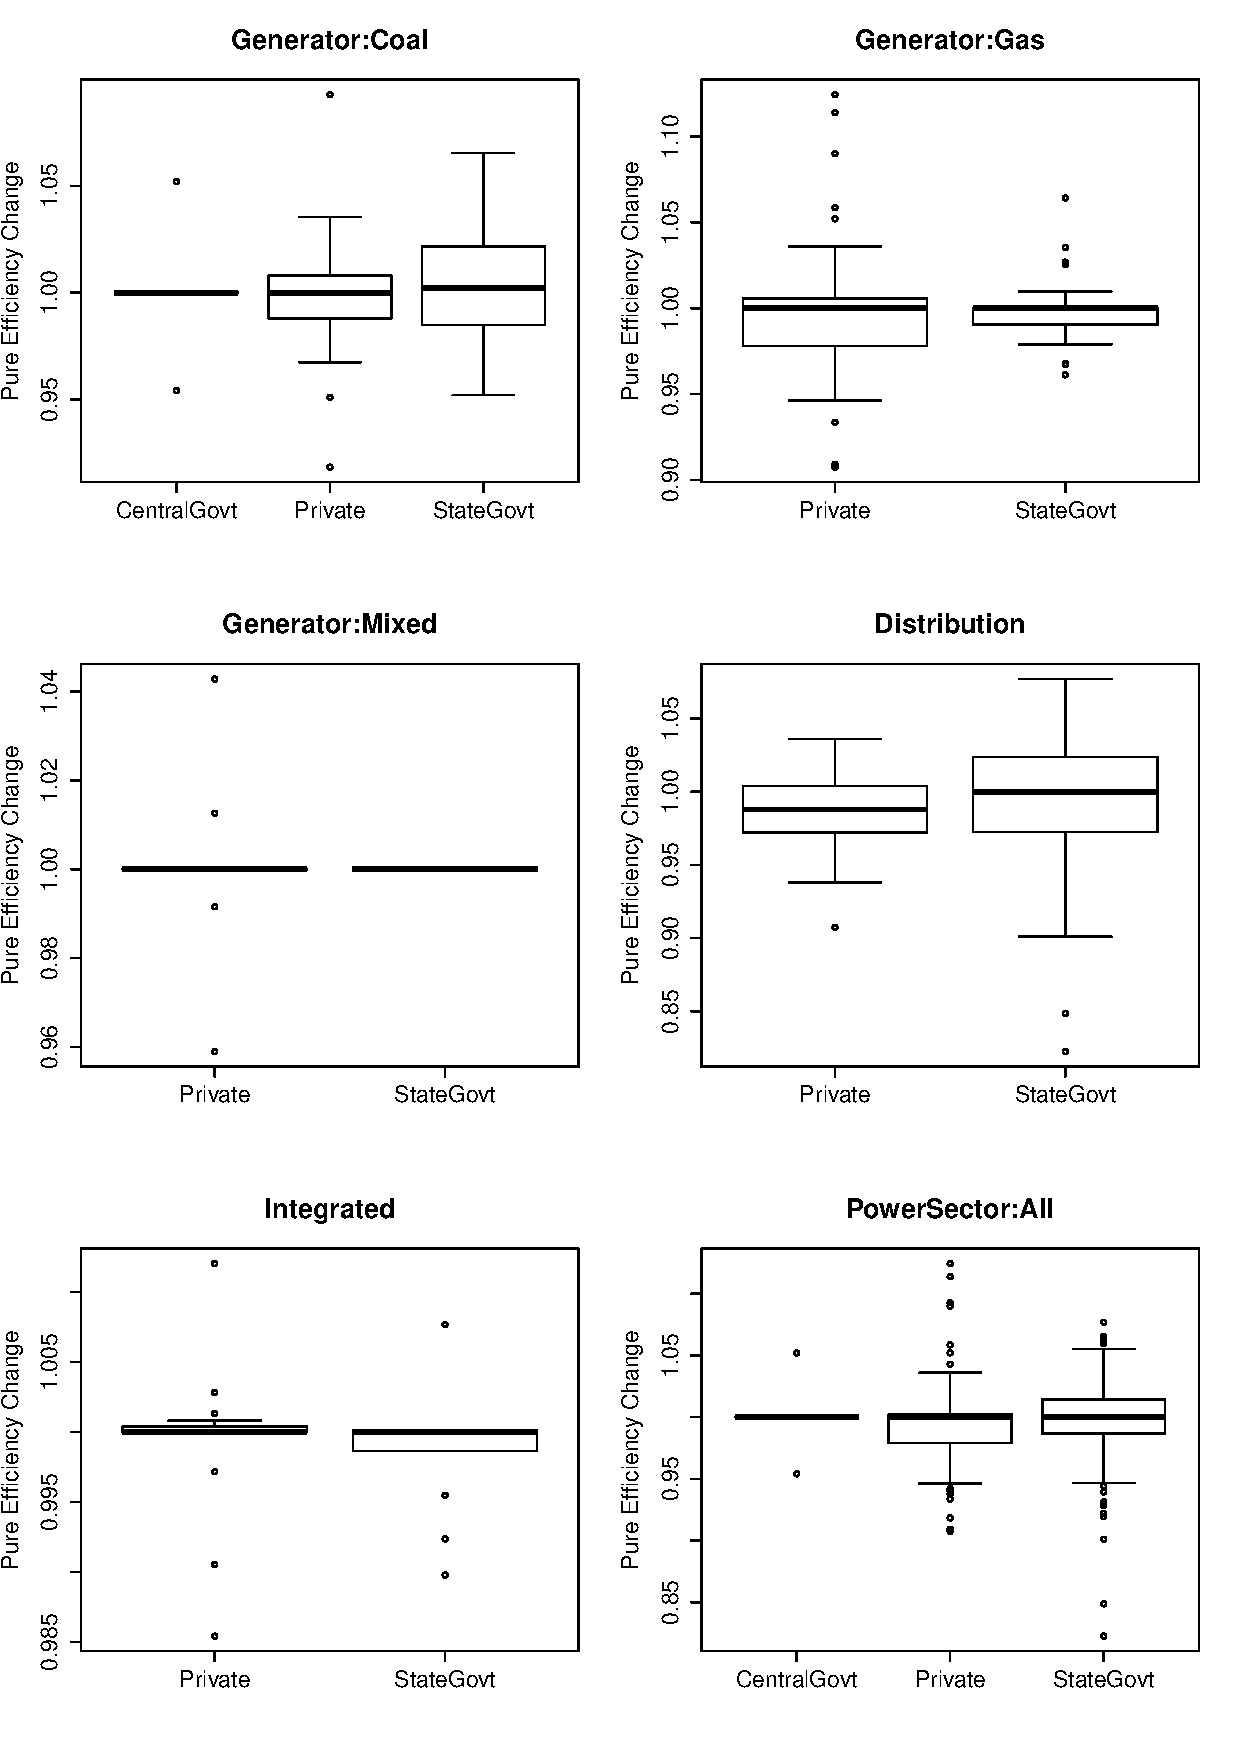
\includegraphics[width=1.00\textwidth]{chapter03/PureEffChange.pdf}
	\label{fig:PureEffChange}
\end{figure}

\begin{figure}[ht]
	\centering
	\caption{Power Sector Scale Change Effect}
		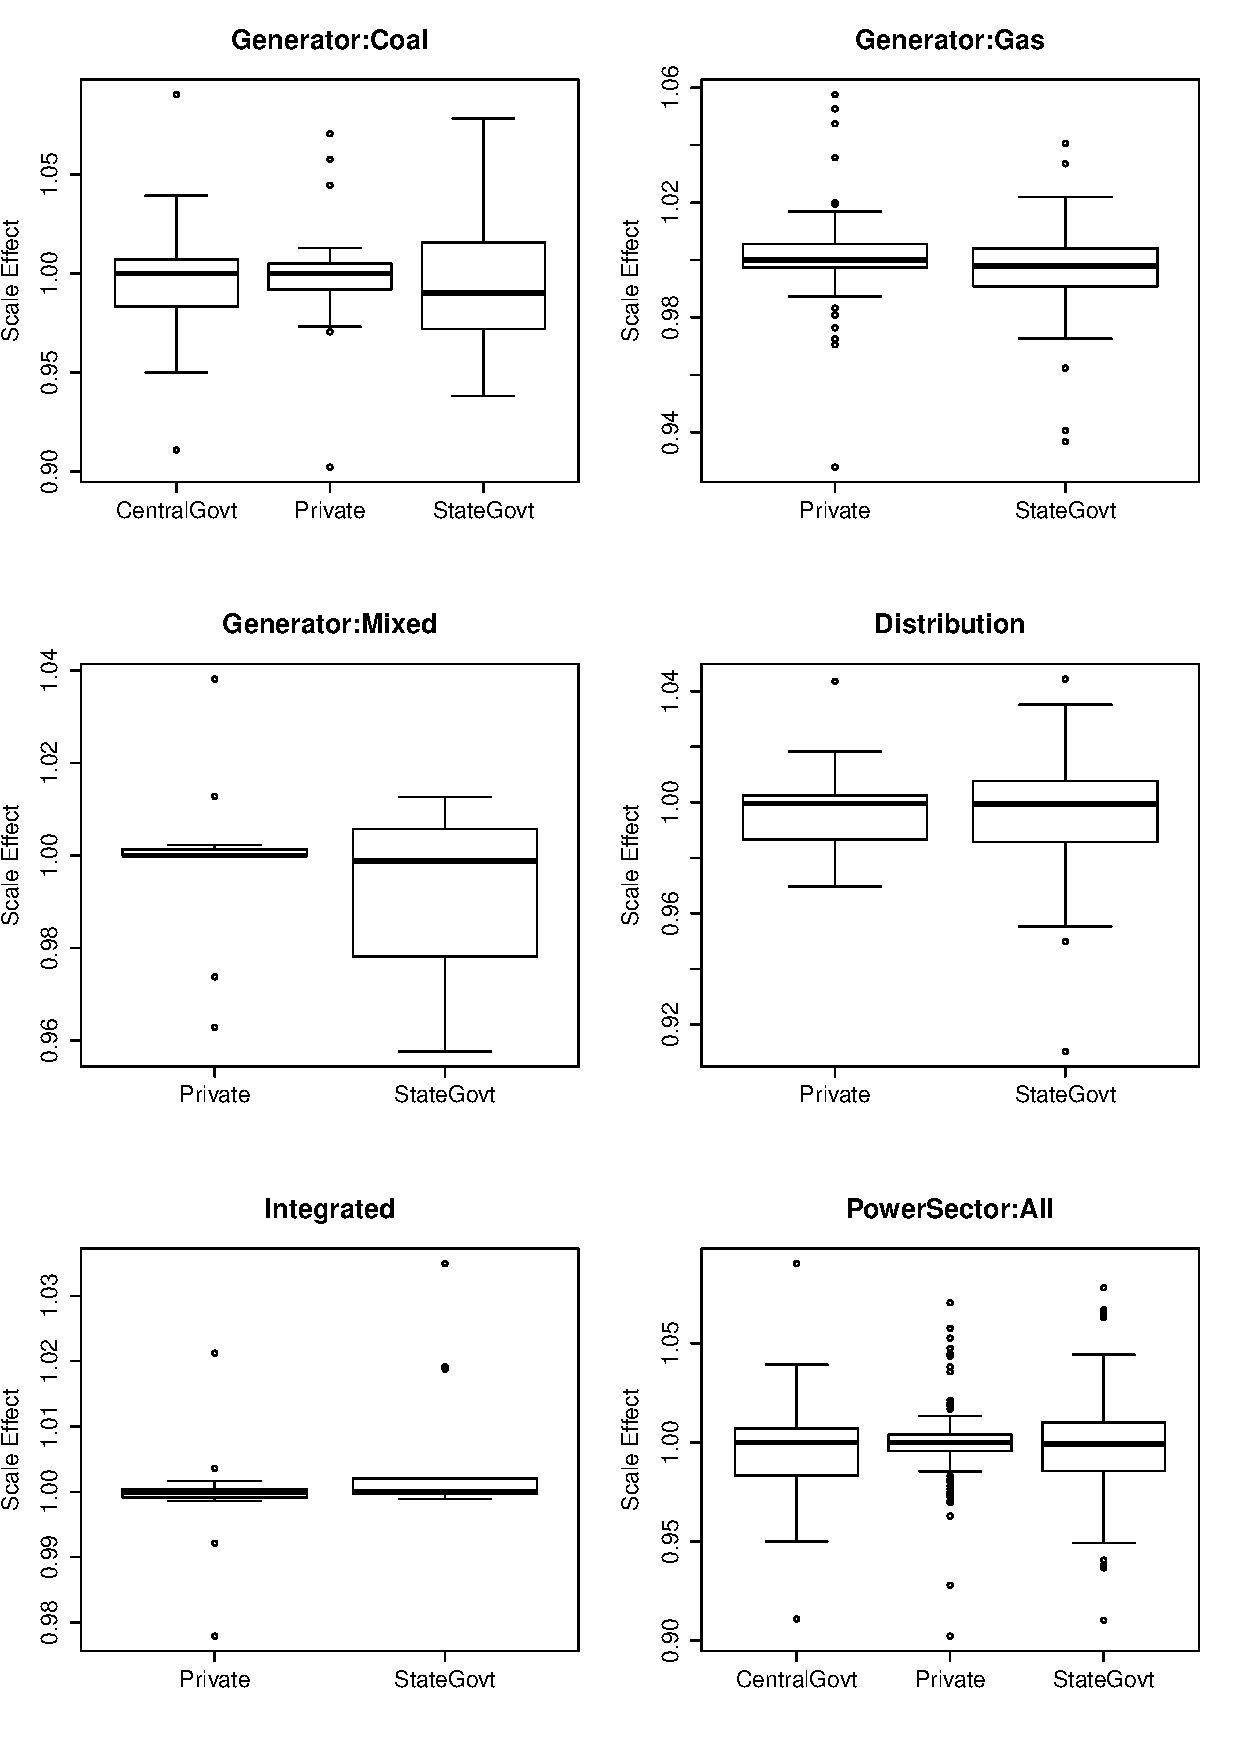
\includegraphics[width=1.00\textwidth]{chapter03/ScaleEffect.pdf}	
	\label{fig:ScaleEffect}
\end{figure}

\begin{figure}[ht]
	\centering
	\caption{Power Sector Pure Technology Change}
		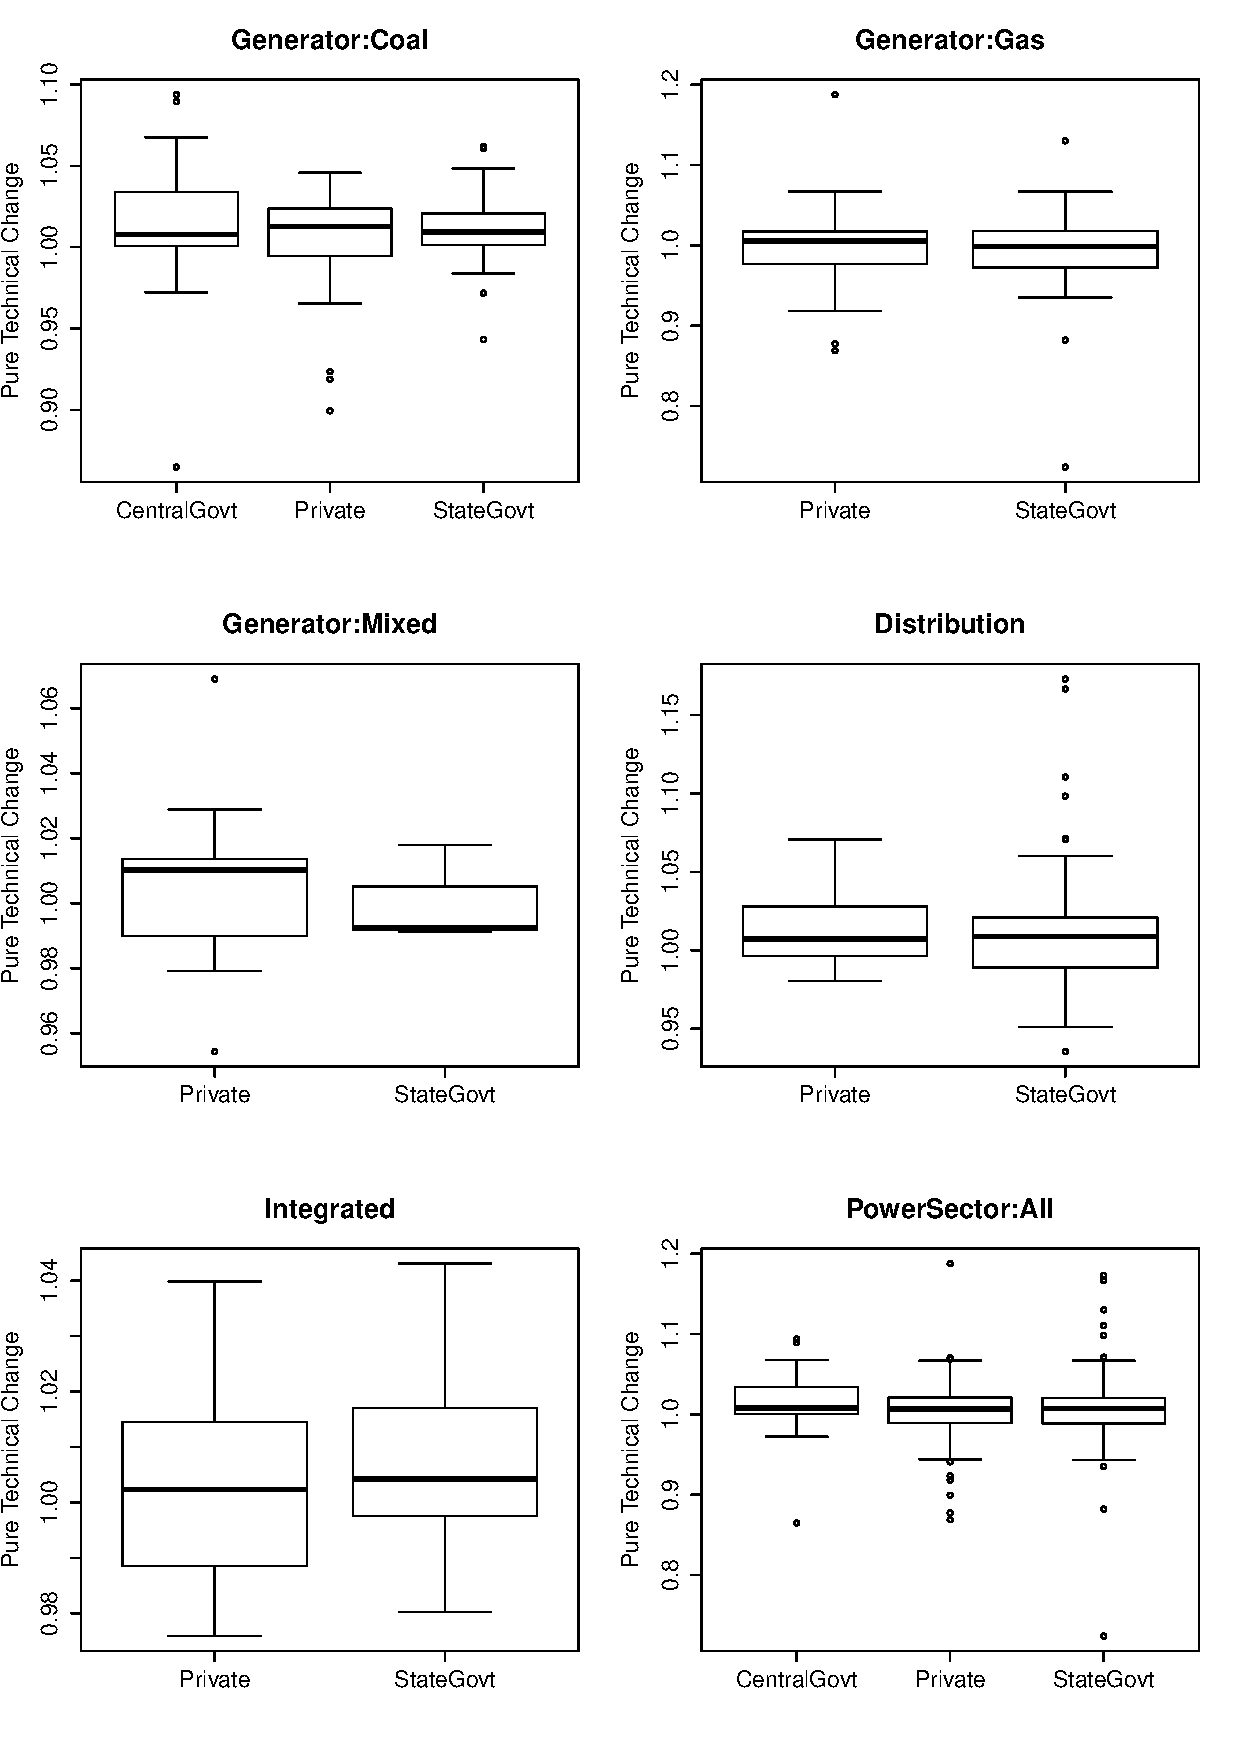
\includegraphics[width=1.00\textwidth]{chapter03/PureTechChange.pdf}
	\label{fig:PureTechChange}
\end{figure}

\begin{figure}[ht]
	\centering
	\caption{Power Sector Technology-Scale Change Effect}
		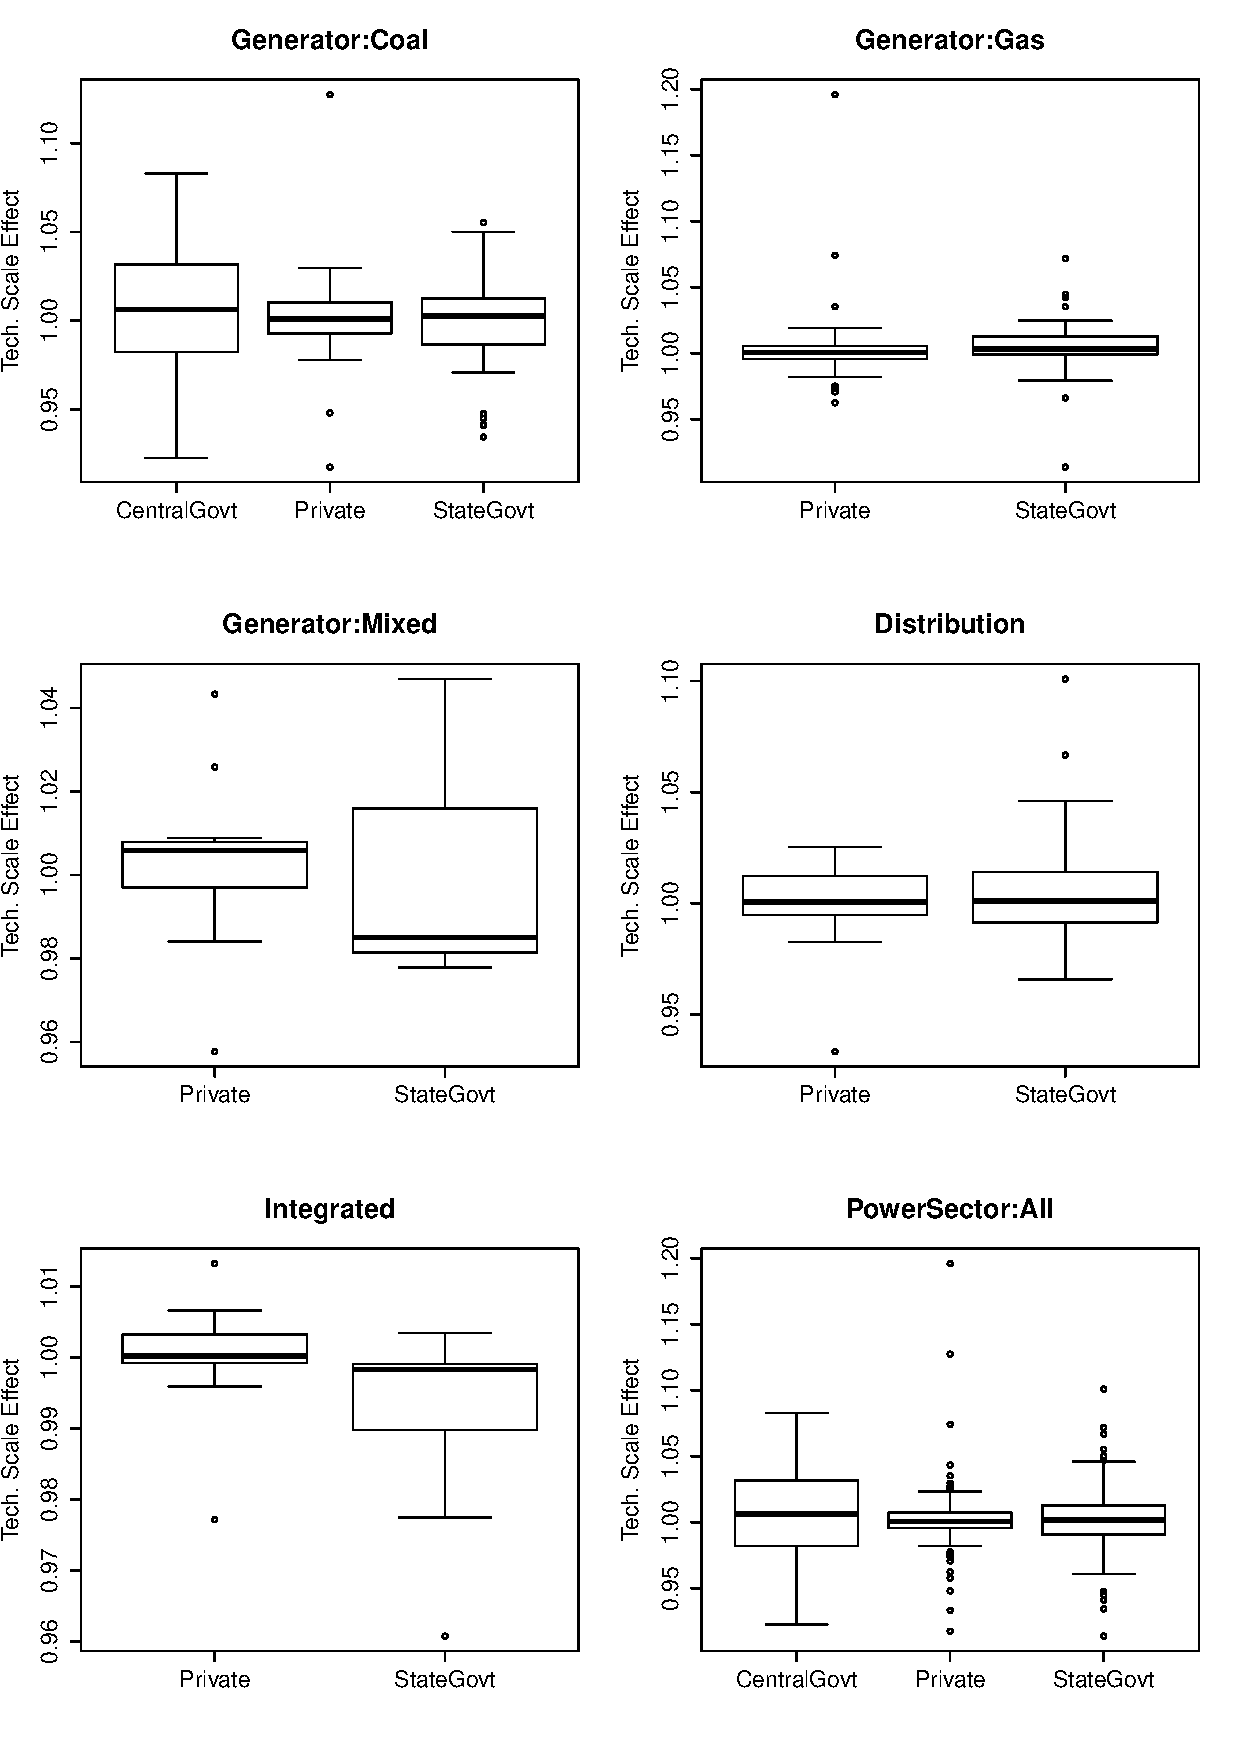
\includegraphics[width=1.00\textwidth]{chapter03/TechScale.pdf}
	\label{fig:TechScale}
\end{figure}


\bibliographystyle{apalike} 
\onehalfspacing
%\singlespacing
\bibliography{chap03refs}
